% Created 2023-09-08 Fri 10:22
\documentclass[9pt, b5paper]{article}
\usepackage{xeCJK}
\usepackage[T1]{fontenc}
\usepackage{bera}
\usepackage[scaled]{beraserif}
\usepackage[scaled]{berasans}
\usepackage[scaled]{beramono}
\usepackage[cache=false]{minted}
\usepackage{xltxtra}
\usepackage{graphicx}
\usepackage{xcolor}
\usepackage{multirow}
\usepackage{multicol}
\usepackage{float}
\usepackage{textcomp}
\usepackage{algorithm}
\usepackage{algorithmic}
\usepackage{latexsym}
\usepackage{natbib}
\usepackage{geometry}
\geometry{left=1.2cm,right=1.2cm,top=1.5cm,bottom=1.2cm}
\usepackage[xetex,colorlinks=true,CJKbookmarks=true,linkcolor=blue,urlcolor=blue,menucolor=blue]{hyperref}
\newminted{common-lisp}{fontsize=\footnotesize} 
\author{deepwaterooo}
\date{\today}
\title{Emacs Configuration}
\hypersetup{
  pdfkeywords={},
  pdfsubject={},
  pdfcreator={Emacs 28.2 (Org mode 8.2.7c)}}
\begin{document}

\maketitle
\tableofcontents


\section{Updates}
\label{sec-1}
\subsection{configuration for org-mode beamer for slides}
\label{sec-1-1}
\begin{itemize}
\item using older version of org-mode because the 2 shorter lines of "\#+BEGIN\_SRC" AND "\#+END\_SRC". DO NOT like newer version two long window width lines.
\item Beamer configuration under older version, I have NOT configued themes for beamer yet, but inline imgs and source code works, basically satisified my usage cases. If I have to configue for new versions, will do when I have time.
\item \textbf{【爱表哥,爱生活!!!任何时候,亲爱的表哥的活宝妹就是一定要、一定会嫁给活宝妹的亲爱的表哥!!!爱表哥,爱生活!!!】}
\end{itemize}
\subsection{configuration for pdf-tools packages}
\label{sec-1-2}

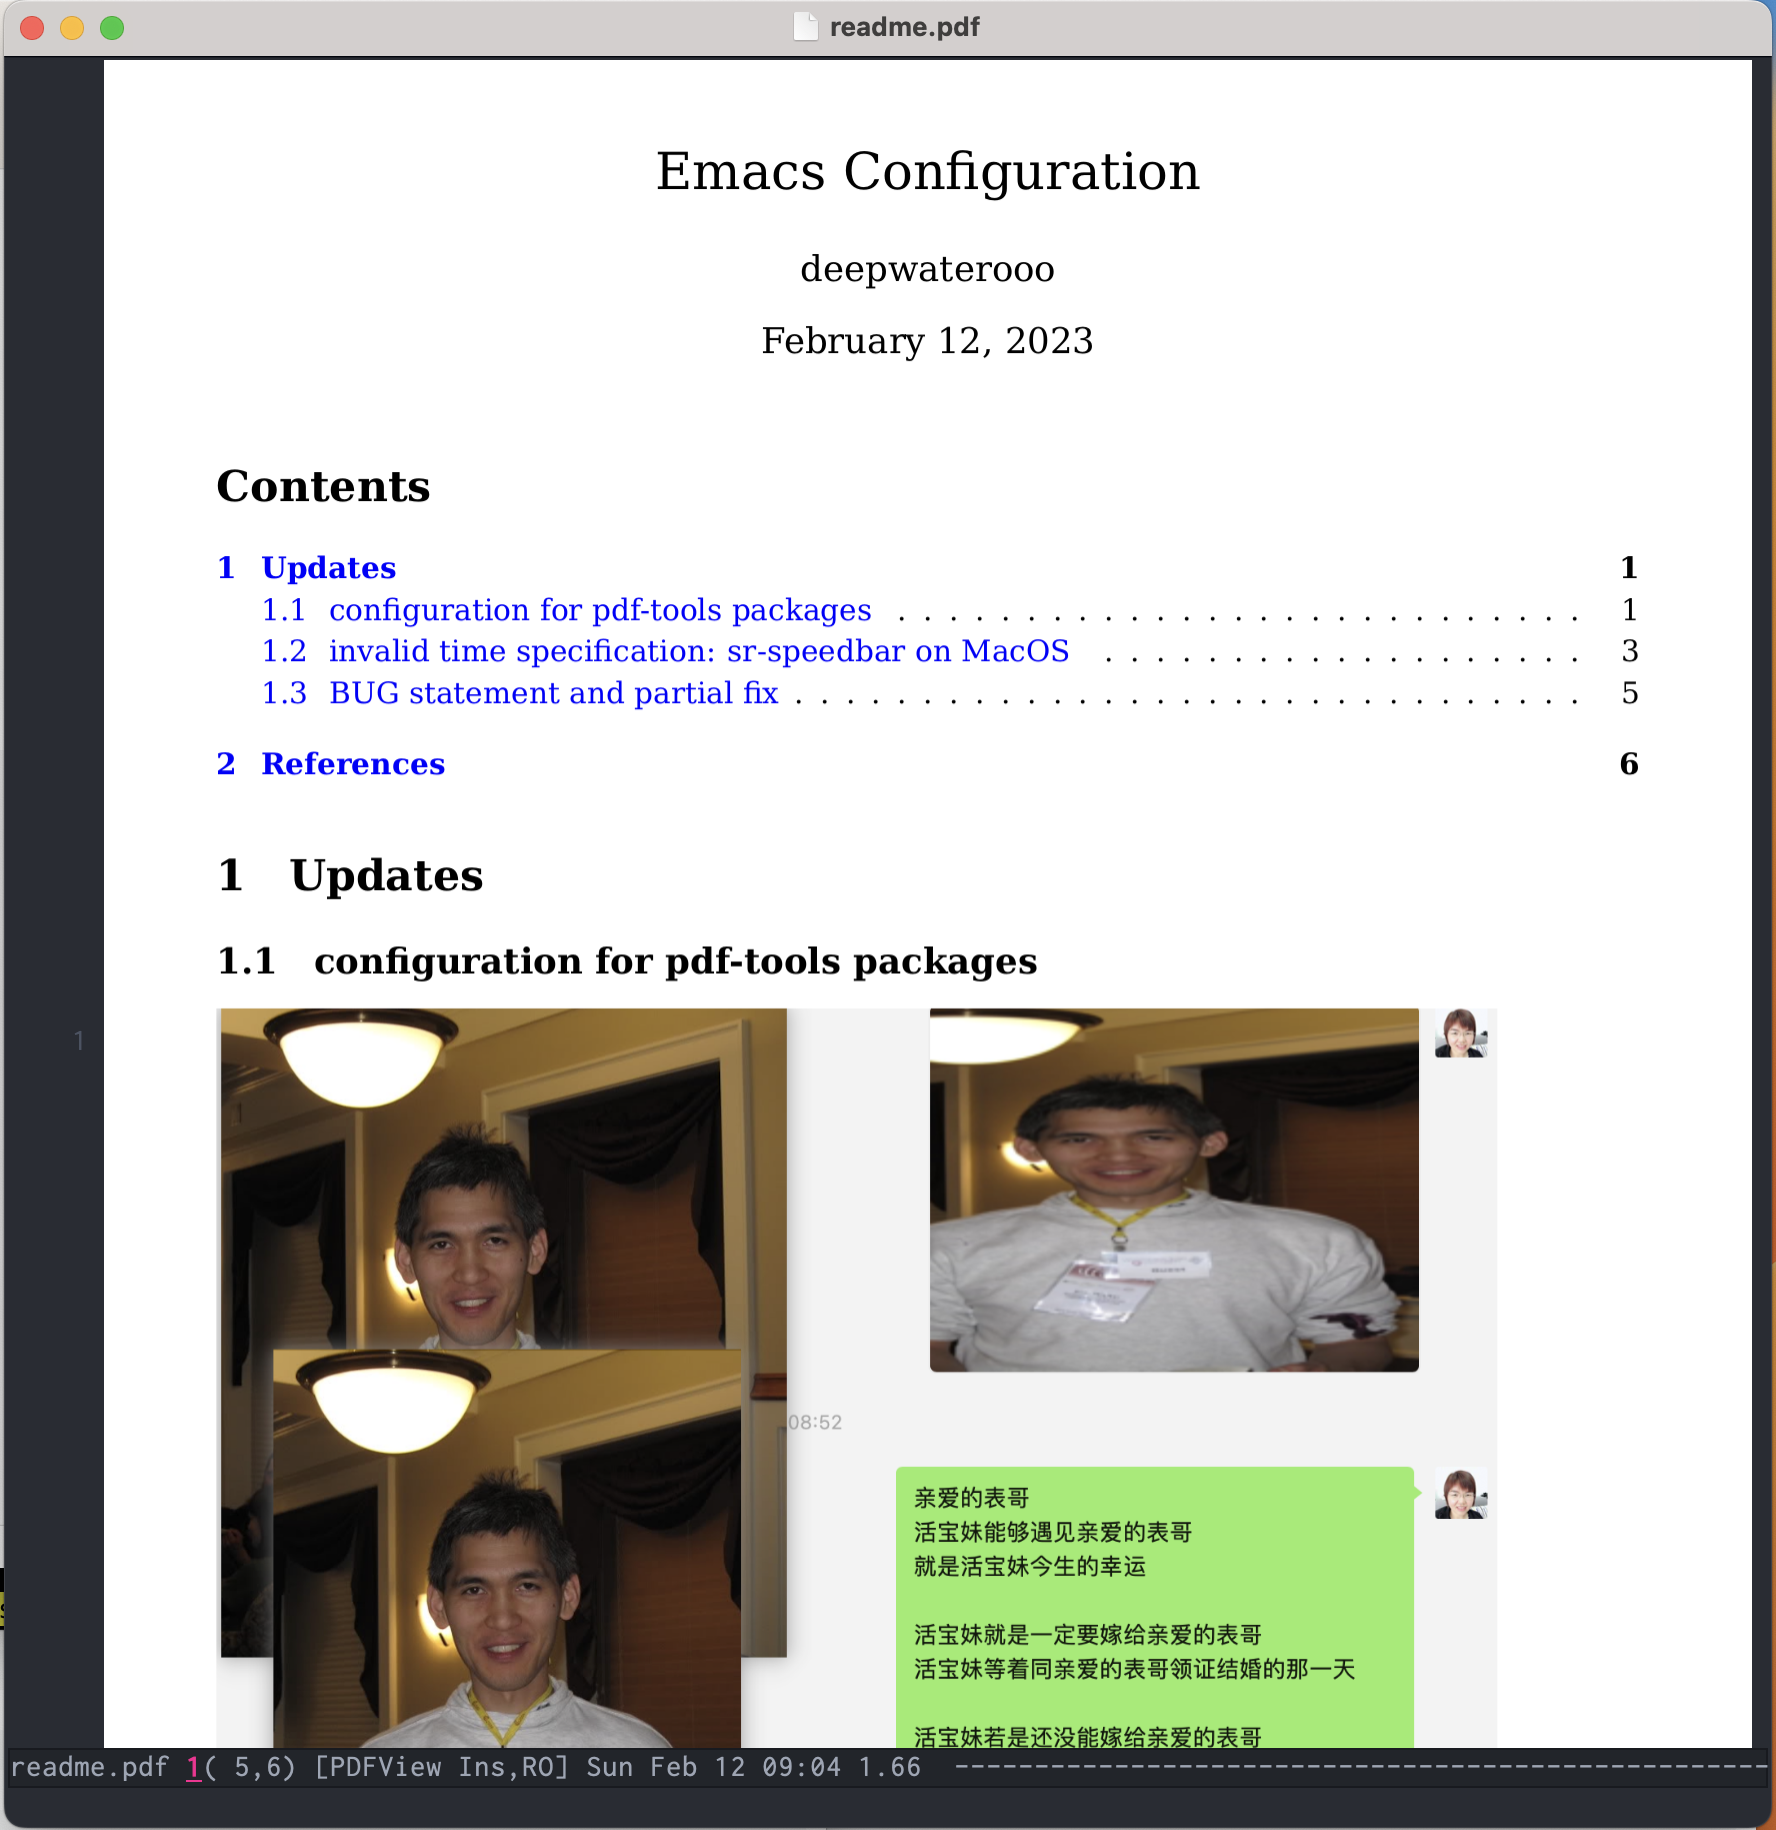
\includegraphics[width=.9\linewidth]{./pic/mememe2.png}
\begin{itemize}
\item pdf viewer noter <==> Skim bi-directional linking configuration on the way, most emacs work is done. Need to learn how to use them though.
\end{itemize}

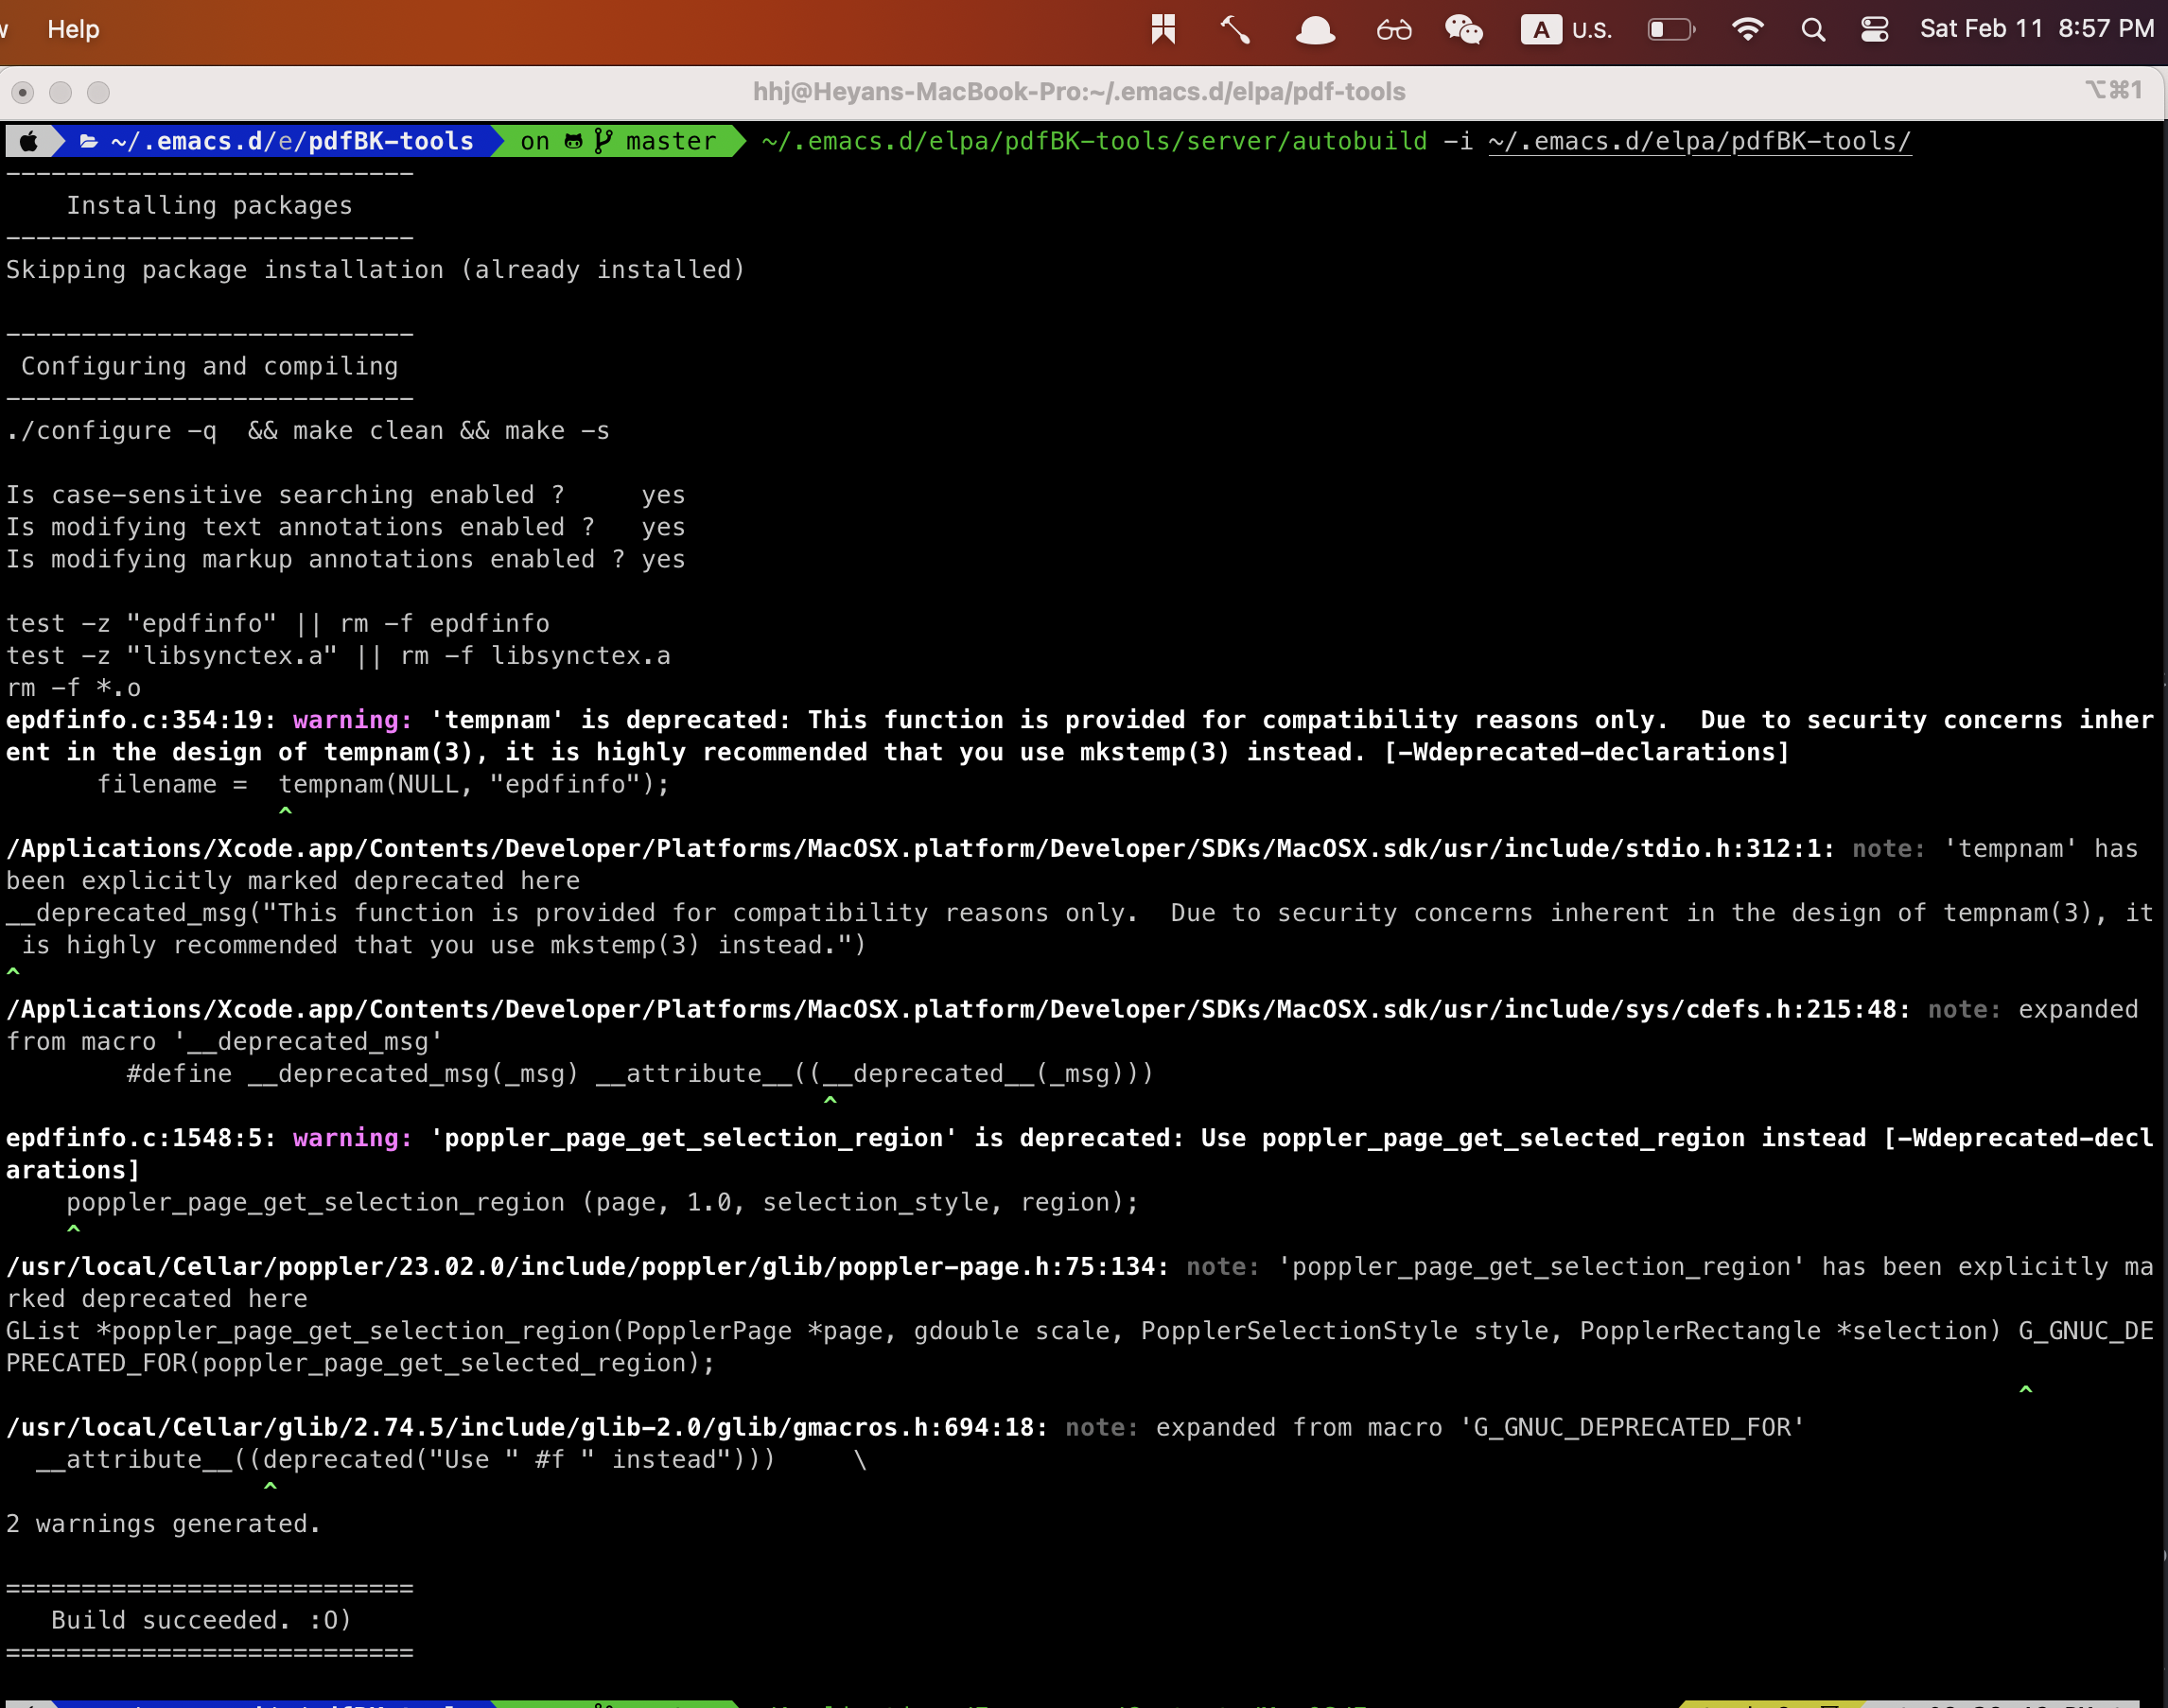
\includegraphics[width=.9\linewidth]{./pic/Snipaste_2023-02-11_20-57-40.png}
\begin{itemize}
\item It has to be configured for M1. But I am still not getting any .tar file yet. 

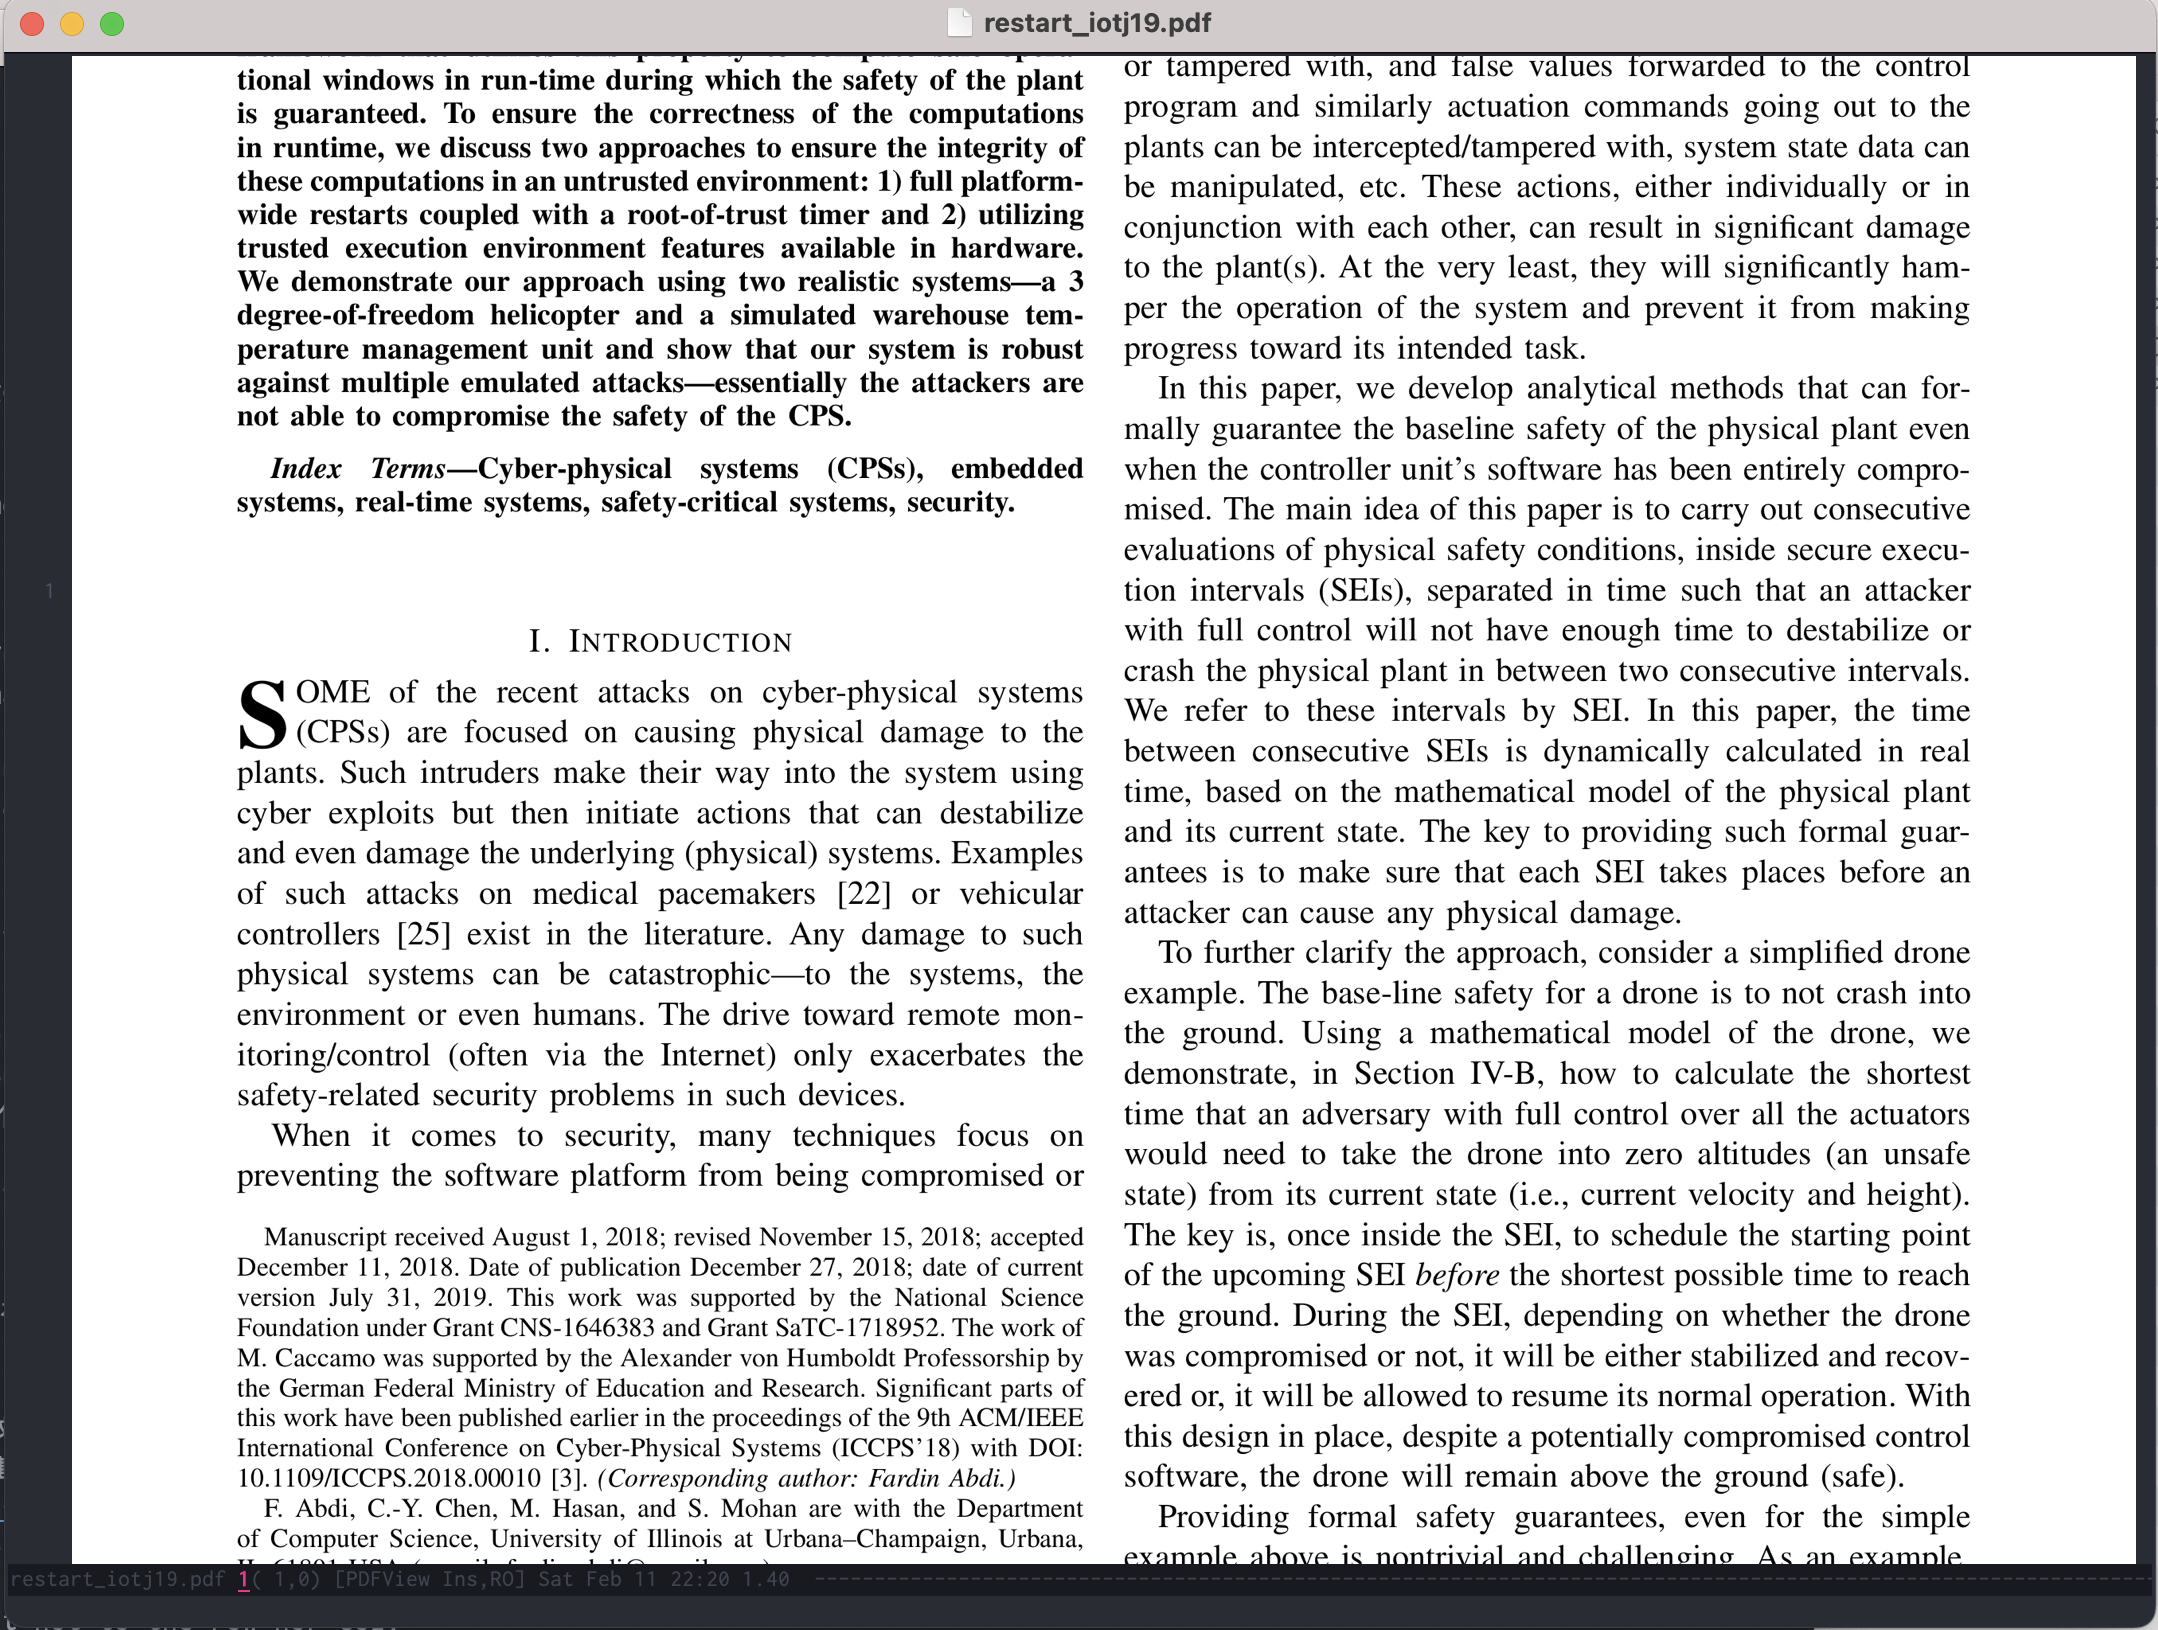
\includegraphics[width=.9\linewidth]{./pic/Snipaste_2023-02-11_22-20-25.png}
\item could customer F5 toggle sr-speedbar, and make sis-mode work. But I do NOT really need sis-mode, only needed macism command line. to help [LOVE MY DEAR COUSIN!!!]
\end{itemize}

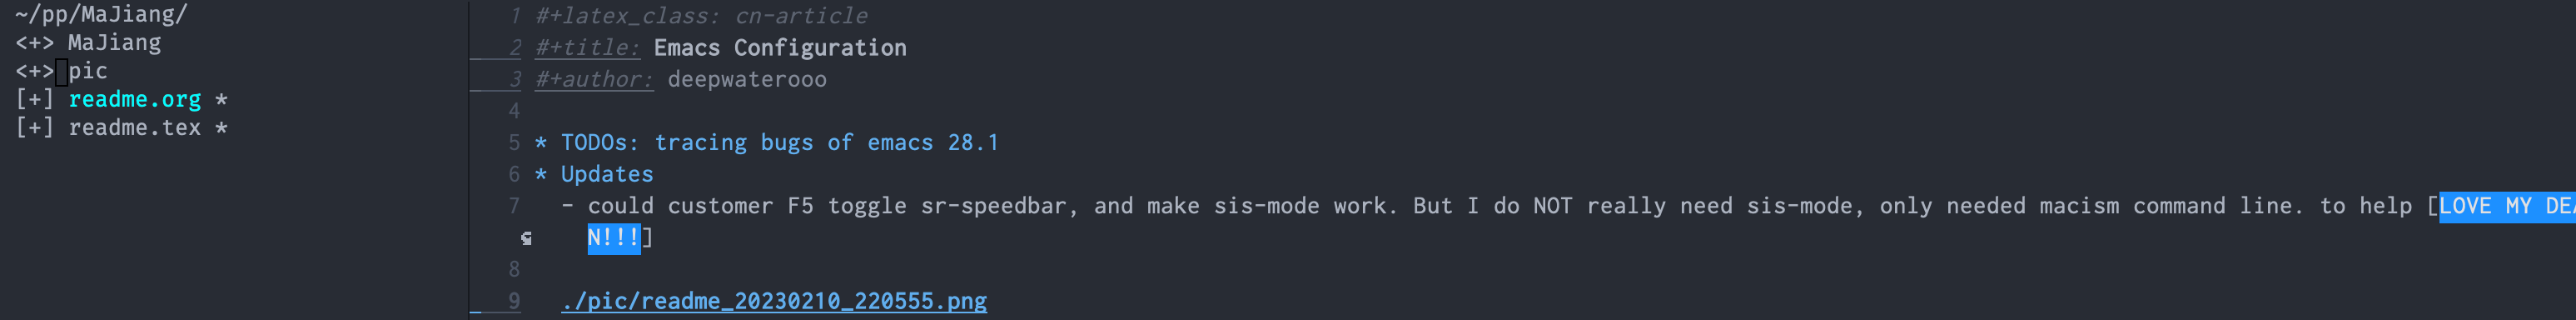
\includegraphics[width=.9\linewidth]{./pic/readme_20230210_221127.png}
\begin{itemize}
\item finally sync up with csharp-mode with tree-sitter, and fixed added the other's that gio-mode etc.
\item Permanently diabled speedbar-edit-file's set-timer function call from Resource files. Do NOT want to see such a bug, don't know how to fix, but disable it and walk around.
\item Now have a relatively barable and stable colorful emacs code editor now, at least for csharp-mode. Relatively satisfied now. Could sit it aside for a while now to focus on projects.
\end{itemize}
\subsection{C/C++ 语言开发环境配置}
\label{sec-1-3}
\begin{itemize}
\item 太久没有用这个了,必须把 emacs 里这个开发的环境配置好。现在用那个什么 init-cc-mode.el
\item \{|\} 的自动扩展开来,我以前不知道怎么回事, java 与 csharp-mode 只能配置好两个中的一个;现在 java 与 csharp-mode 与 cc-mode 似乎都能自动扩展。当初是怎么回事呢?等改天用多了看它还会不会再抛锚抛错。。。先把自己其它 mode 里【中英文】切换注释等常用功能銉转到这个 mode 里来,没问题。这些简单功能都容易实现。
\end{itemize}
\subsection{{\bfseries\sffamily emacs} 1 initiliation bug}
\label{sec-1-4}
\begin{itemize}
\item TODO: 需要将Rime 动态库构建成适配配置到 arm64-arch 版本。它性能我电脑的整体性能。
\end{itemize}
\section{Emacs x86\_64 vs arm64-arch, and System Rime input method: \textbf{【TODO: 现在应该可以系统更新了!!】}}
\label{sec-2}
\begin{itemize}
\item 因为Macbook 下的 Rime 输入法支持arm 的构建已经好了,我应该可以 \textbf{【构建出 arm64-arch 的Rime 动态库给 emacs 用】}
\item Rime 安装链接:\url{https://github.com/rime/squirrel/blob/master/INSTALL.md}
\item 把 emacs 升级为 arm64-arch
\item 把 arm64-arch 的 emacs 版本pyim 配置好
\item 把 appcode 重新安装 arm64-arch 版本,应该就可以与 arm64-arch 版本的 emacs 自由跳转了。而不必再是 X86\_64 版本的。
\item \textbf{【总结】} :安装 arm64-arch 版本,是与自己笔记本硬件更好地配合提升效率。
\begin{itemize}
\item 但过程繁琐,仍然不能达到 \textbf{【亲爱的表哥的活宝妹,实时想要动态更改词库,实时想要更新动态库给 emacs 用的需求!】}
\item 这系列更新包括:Rime-arm64 版本安装与自己构建、emacs 删除与重新安装与 pyim 配置, appcode 的删除与再安装。前两个应用都可能出问题。。。若真出问题,就把自己的配置摧毁掉了。。。
\item 我其实只要去解决:【亲爱的表哥的活宝妹,怎么才能手动构建 Rime 的动态词库?】只要我能手动构建更新后词库的动态库,我就满足了自己的使用需求。
\begin{itemize}
\item 【难点:】这是别人输入法的精华。虽然只改了一个最小的脚本错误,但是正如全中文网没人会告诉你别人输入法的精华、没有贴子真正会涉及这些精华(细节的构建步骤,只有一个几年前的老贴子不 work: \url{https://hackmd.io/@PhahTaigi/r1tlmy0cV),所有的都是去抓现成的缺省版本的。就当自己想要了解和深入中文输入法更进一步。留这个兴趣点在这里。改天有时间、有机会再看。细节上,就是Rime} 的 boost 库可能也没有能够找全,该生成的文件没能全部生成。也可能是因为现在系统 arm64-arch 硬件与 x86\_64 Rime 的库不匹配?可是我试 x86\_64 之前,先试过本地 arm64-arch 版本,也没能生成。改天再看。(可以参考 Rime 提供的不完整步骤:\url{https://github.com/rime/librime/blob/master/README-mac.md} 和一个用户M1 的步骤: \url{https://www.bilibili.com/read/cv9664366/}. 另Rime M1 手动构建步骤说明:\url{https://github.com/rime/squirrel/blob/master/INSTALL.md})
\end{itemize}
\item 折腾了大半个下午,仍然同先前一样构建不出来,只是感觉比前几个月似乎理解得更深刻一点儿。说明今天下午大改前的考虑是对的,看起来狠容易的动态库构建,没人自己手动构建,只有亲爱的表哥的活宝妹突发奇想,觉得可能可以有效更新词库。实际因素可能还有狠多。这个思路暂时放下。
\end{itemize}
\item 【重点:上次我的 emacs 升级,为什么我不能把它直接升级到 arm 版本来着?那个 csharp-mode 的循环问题不是早解决了?!!!可以再试下? NO, not yet.】
\begin{itemize}
\item 现和使用的 x86\_64 版本,当初是为了安装 pyim 吗?如果是这样,我不应该再有任何的变化,就意味着我无法从 appcode 中打开当前 emacs 的 buffer 文件(因为 emacs 的 x86\_64 版本限制了其正常找到 appcode 所依赖的 arm64-arch 环境?这个可以试着找下是否有解决方案);
\item 而如果 pyim 可以 workwith arm 版本,我就可以安装 arm64-arch 版本,可能就可以从 appcode 中打开当前 emacs 的 buffer 文件了。
\item 我要再试一遍?【现在还不能够试,在我还不能够构建和安装出 rime 系统输入法的 arm64-arch 版本动态库之前(这个输入法,现系统所安装的是 x86\_64 版本的),我安装 arm64-arch 版本的 emacs ,我的pyim 将不可以用(找不到对应版本的 rime 动态库),因为我构建不出 arm64-arch 版本的 pyim 所依赖的动态库。所以将现在的 emacs 委屈成了 x86\_64 版本的,也因为这样,我的 emacs 无法正常加载 arm 版本的 appcode 所依赖的动态库,所以无法从 emacs 中直接在 appcode 中打开当前 buffer 文件。】
\item 可以 walk-around 的解决办法是:安装 x86-64 版本的 appcode. 【在自己能够想方设法构建出 arm 版本的 rime 动态库之前,先用这个版本,可以满足自已的基本跳转需求】
\end{itemize}
\end{itemize}

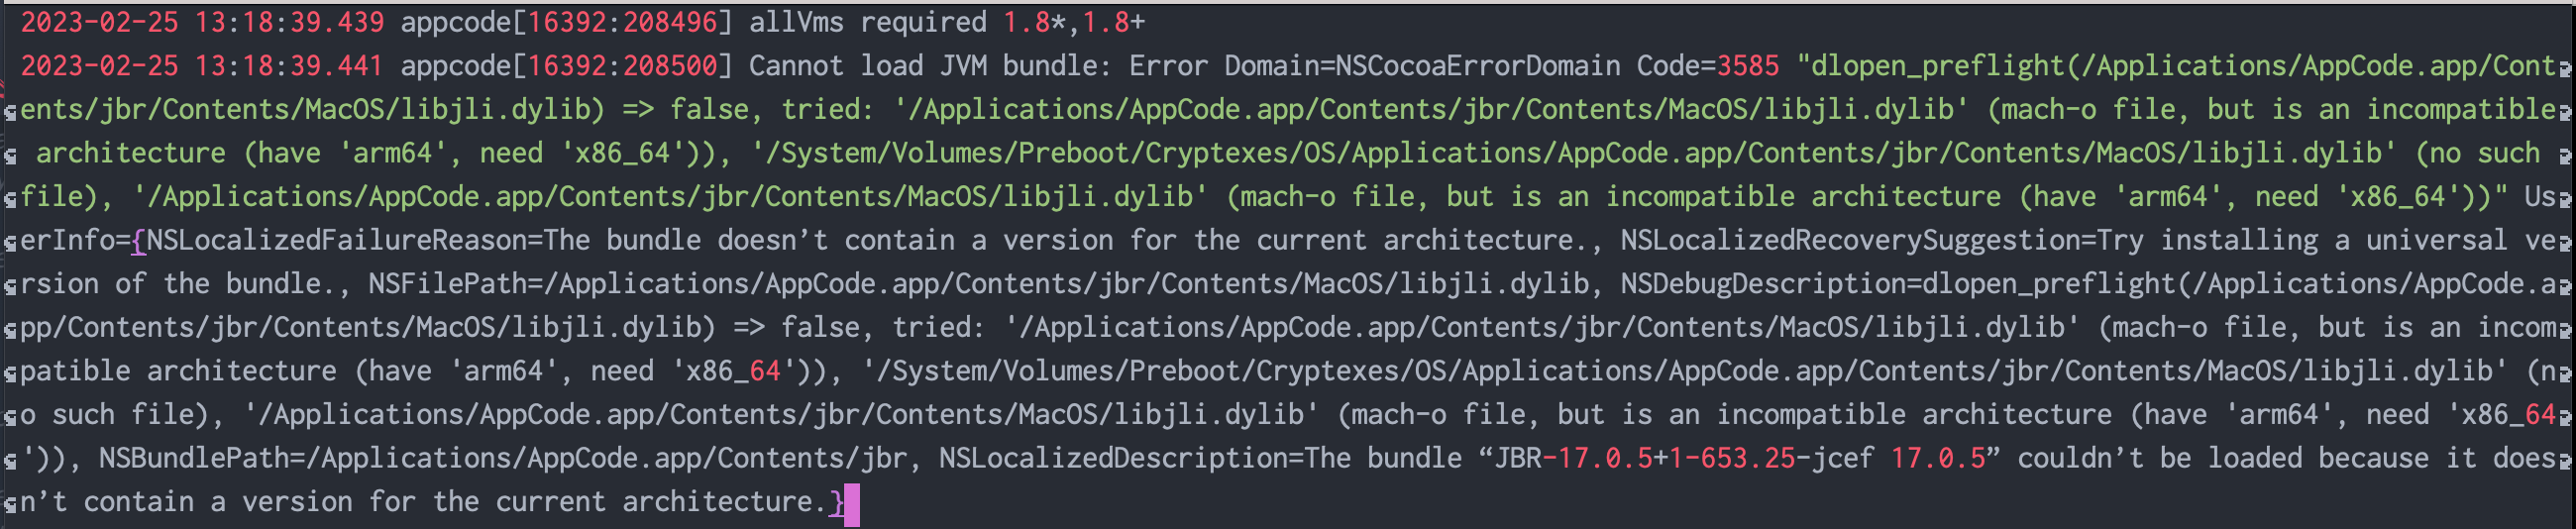
\includegraphics[width=.9\linewidth]{./pic/readme_20230225_132052.png}
\begin{itemize}
\item 有试过, boost 的步骤基本能够完成,但是构建第三方库时的 cmake 与 xcode-clang++ 还有很多 arm 相关的问题待解。
\item 那么我现在有个迫切需要:就是能够自己构建 arm64-arch 版本的 rime 输入法( 至少是能够编译出它的动态库吧?!!!):现在找到的参考如下: 
\begin{itemize}
\item 现在 emacs 使用的是 28.2 X86\_64 版本。我 \textbf{【想要动态手动更新Rime 五笔第三方库】} 。可是我忘记当初几个月之前,我是怎么添加这个动态库给 emacs 使用的了。会找一找。也可能再尝试能否构建出 arm 版本的第三方库。
\begin{itemize}
\item 有个教程,这里也简要记一下过程,免得自己总忘记:大致过程:
\end{itemize}
\end{itemize}
\item 把Rime 的重新部署好的动态库,复制到 emacs 的Rime 第三方适配库 librime 特定目录下
\item emacs 的Rime 第三方适配库 librime 下,生成Macbook 系统可用的用户第三方库
\item 再配置 emacs 什么的就可以了。加个截图:【爱表哥,爱生活!!!任何时候,亲爱的表哥的活宝妹,就是一定要嫁给亲爱的表哥!!爱表哥,爱生活!!!】
\end{itemize}

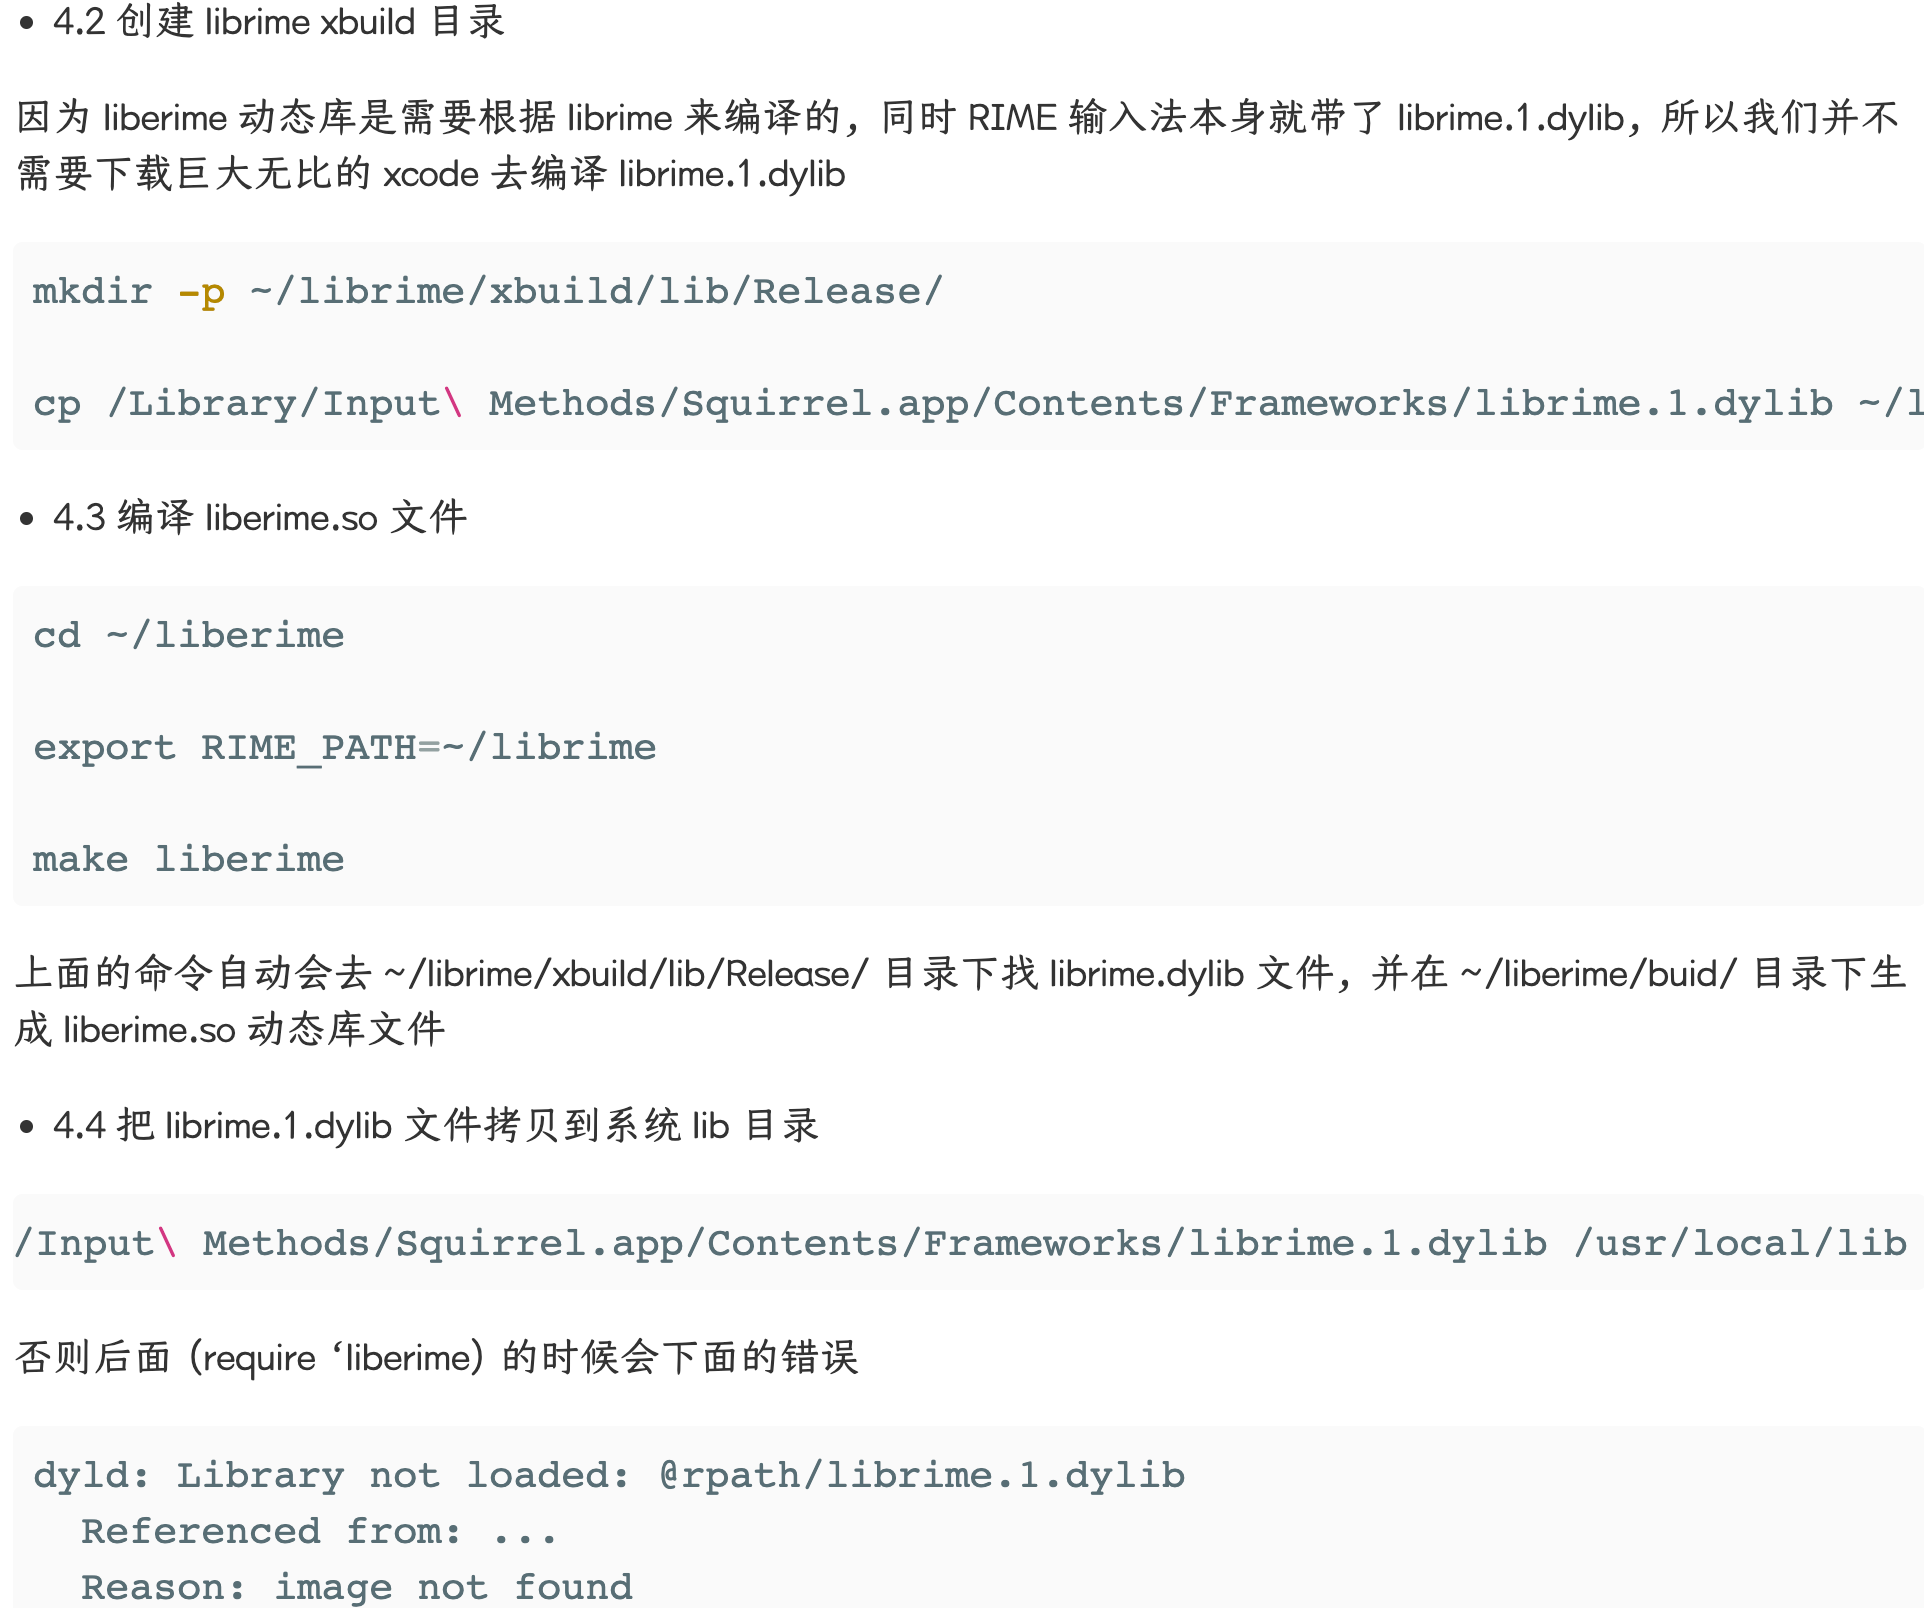
\includegraphics[width=.9\linewidth]{./pic/readme_20230718_111929.png}

\begin{itemize}
\item \url{https://www.bilibili.com/read/cv9664366?from=search}
\item 但是按照上面的步骤,目前理解消化不够,安装不好。注意,这里用到的 MacOS 下在的库是: \url{https://github.com/rime/squirrel} 但是我仍然构建不出那个动态库
\item 如些发现,原来,所谓 rime macOS 下的输入法构建,原来是 MacOS 下的平台应用,正是我可以学习的地方。终于是半只脚往输入法的坑里踏:
\begin{itemize}
\item \url{https://www.logcg.com/archives/2078.html}. 这些都可以成为日后自己学习和开发的参考
\end{itemize}

\item emacs 27.1 for emacs-rime input methods. one bug to be fixed. 

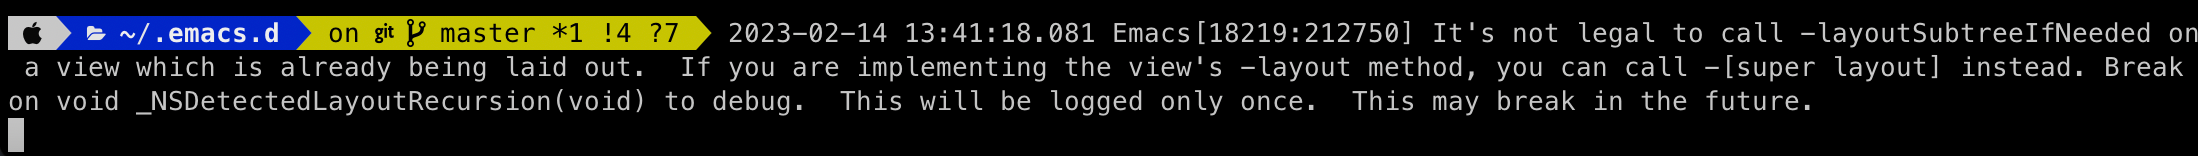
\includegraphics[width=.9\linewidth]{./pic/readme_20230214_134351.png}
\item this affect me access to current terminal, needs to be fixed later.
\item after having updated swift-mode, color-theme for swift mode is much better now.
\end{itemize}
\subsection{configue pyim wubi input method emacs-rime, works like a charm!}
\label{sec-2-1}
\begin{itemize}
\item 现在最大的缺点是:我无法使用自已魔改过的个性化字库,姓名住圵等等,活宝妹,亲爱的表哥,等等。但其它也算是基本清单了,再不折腾它了。花了太多的时间在这个上面。所以现在输入法还算是基本清单的。
\begin{itemize}
\item 两套:系统的,与 emacs 里自带的。目前的中英文转换只使用一个探针,过多会存在过灵的总是,某些情况下被禁用中文,就会更麻烦,不如它没有那么灵。爱亲爱的表哥,活宝妹一定要嫁的亲爱的表哥!!!
\end{itemize}
\item 它具备以空格来区分中英文输入法的功能,但不能与中文下半角配合使用。也就是,它具备了我现在所使用过的 sis 下的自动中英文之间以一个空格为单位自动切换,但我无法使用中文下半角标点。
\item 它除了使用了系统输入法的字库,其它所有好用的配置一个也不能用(我只能拦截一个最常用的半角,仍然是不方便的),现在只是可以选詞了而已,却不能使用其它中文下输入英文标点符号等
\item 我中文下使用英语标点:主要是 org-mode 打头的 -*. 等,它可以检测到,自动化到,还是方便的
\end{itemize}
\subsection{invalid time specification: sr-speedbar on MacOS}
\label{sec-2-2}
\begin{itemize}
\item I don't like this bug, and I belive I do NOT really using any timer for auto-refresh in my speedbar. So I ended up by disabling the (speedbar-edit-file() func, which is frequently bug trigered) setting timer part from /Applications/Emacs.app/Contents/Resources/lisp/speedbar.el.gz, and recompile the file. The bug was gone. And I could deal with csharp-mode's fontify bug.
\item newer debugging infos, concernibg about sr-speedbar.el file. Have NOT been able to trace down for today.
\end{itemize}

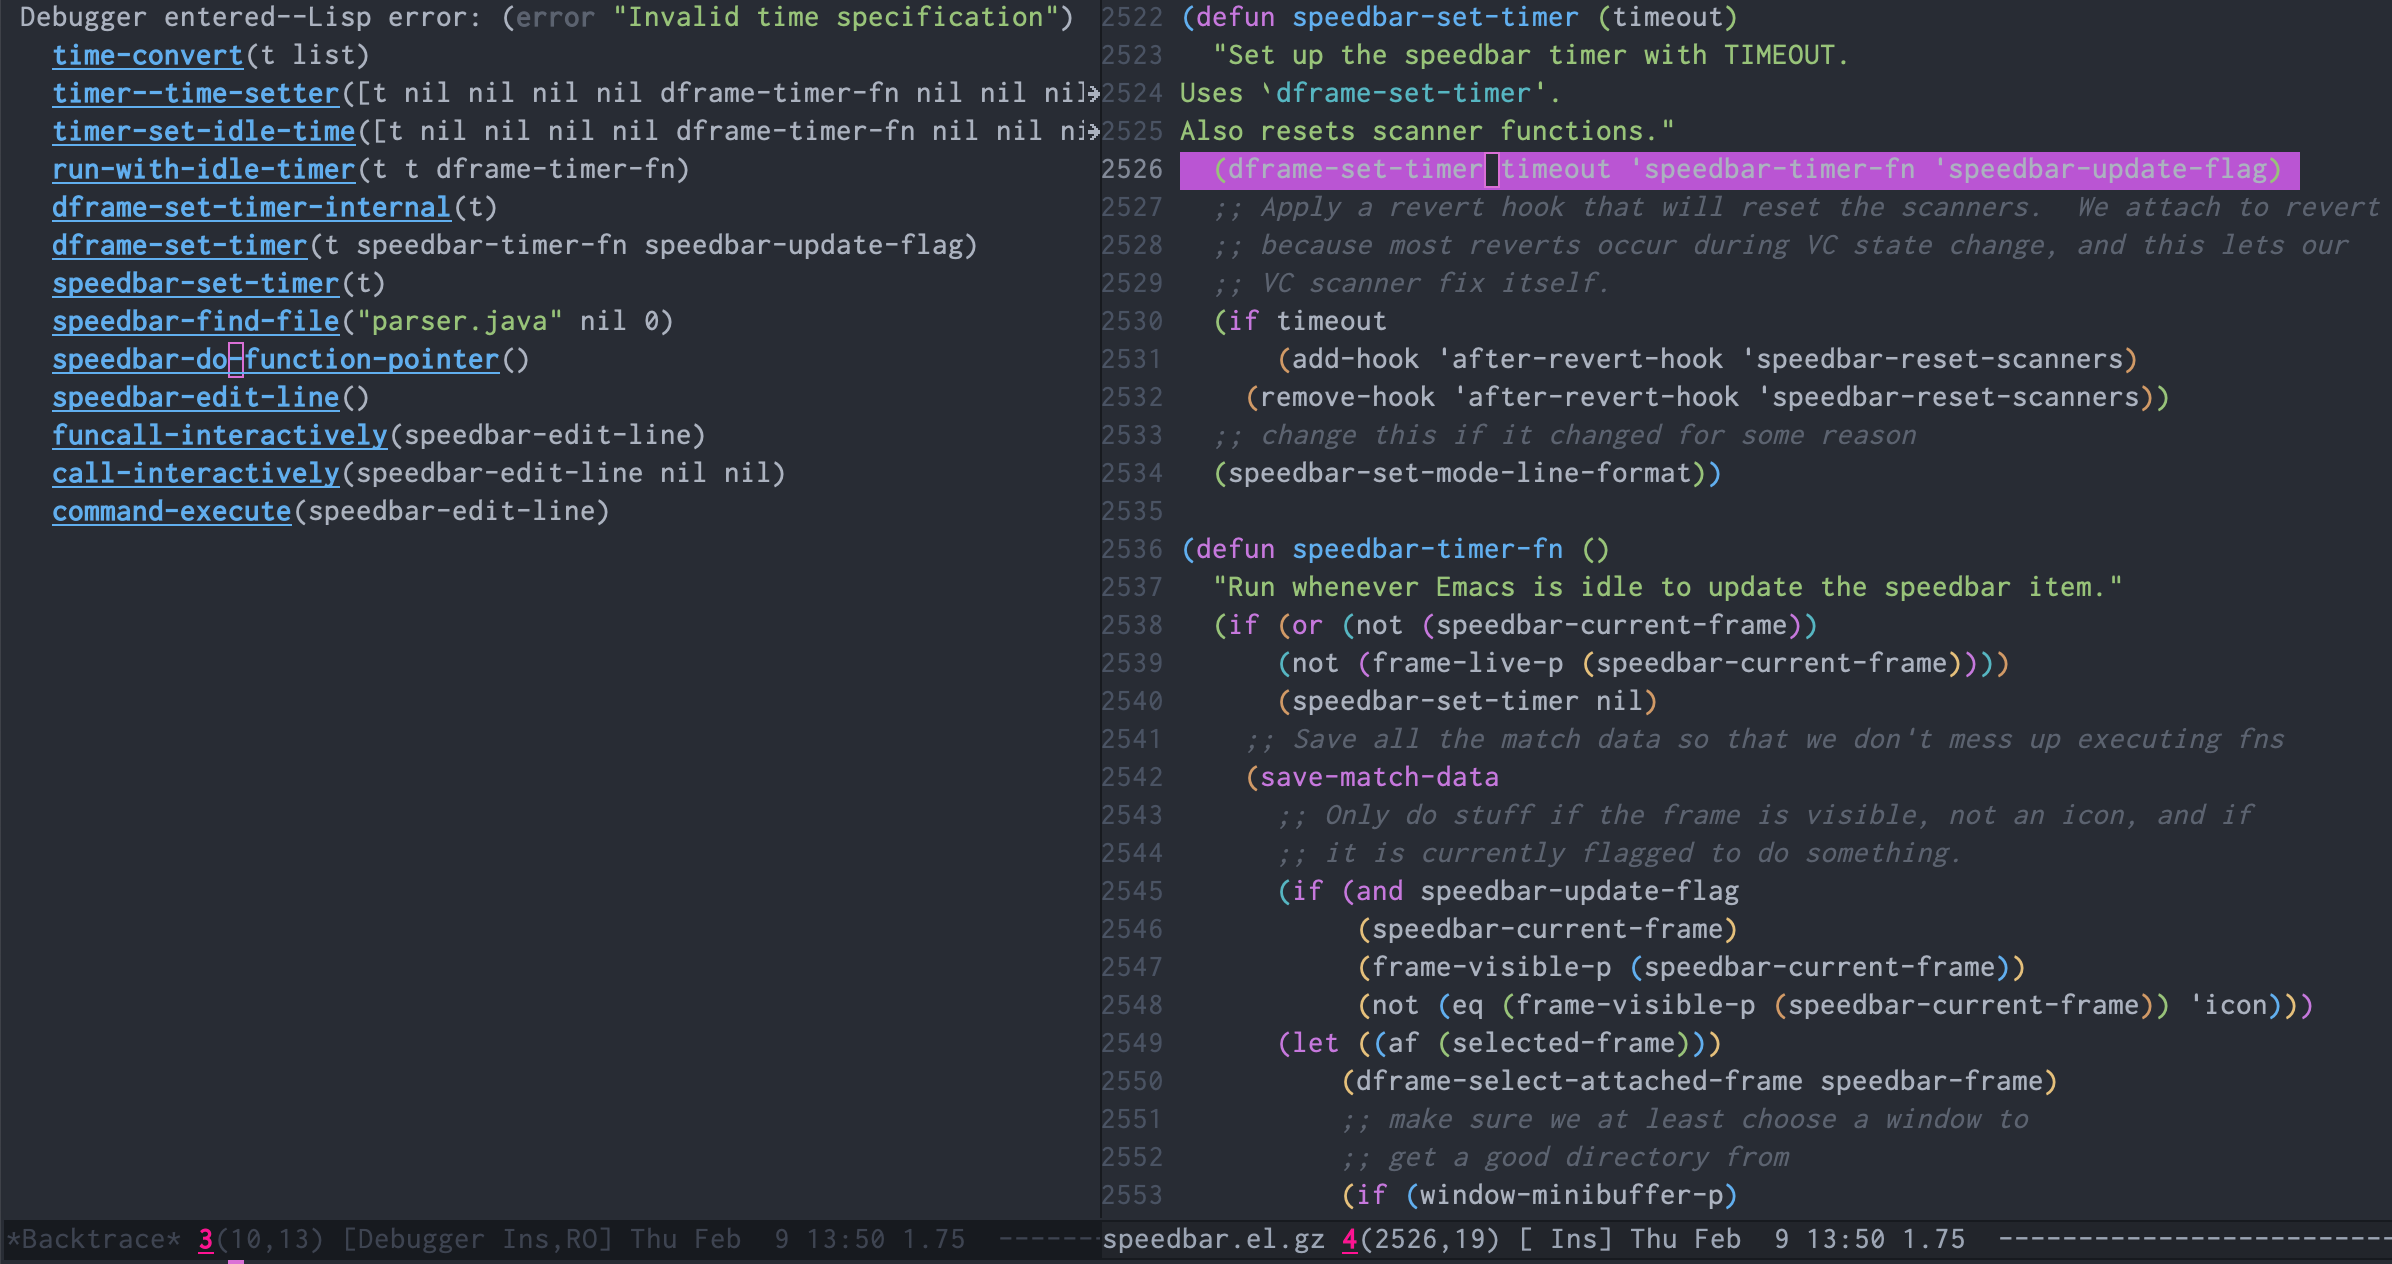
\includegraphics[width=.9\linewidth]{./pic/readme_20230209_135039.png}
\begin{itemize}
\item 好像是macOS系统常常存在的 bug,两年了关了又开,开了再关\ldots{}\ldots{}
\item \url{https://github.com/remacs/remacs/issues/845}
\item get cmake work later, not urgent though.Complete
\item babel org-mode so I don't have to copy from specific babeled source org-mode files in order for chinese characters to work.
\item Installed my emacs of version 28.1. But there is a bug of any verison emacs > 27.1, and I am NOT able to find a installable emacs 27.1 version any more.
\item 不同电脑架构上可能因为架构的不同,可以可能可以有某些优化.又照一个单做了一遍,似乎没有出错. \url{https://goykhman.ca/gene/blog/2022/2022-04-10-emacs-28.1-on-m1.html}
\item 但是我没有没能加入那个补丁包.暂时没能想好怎么加入那个补丁包. ( \textbf{todo: 改天可以尝试再把这个补丁包加进去} )
\item 因为构建是在原有现有的 mac 28.1.1版本上构建的.所以改动什么,或是不曾改变,又或者改不了不影响明显功能都是无从知晓的,但是它最后的两个步骤的验证都是成功的,应该还是构建成功了吧?
\end{itemize}

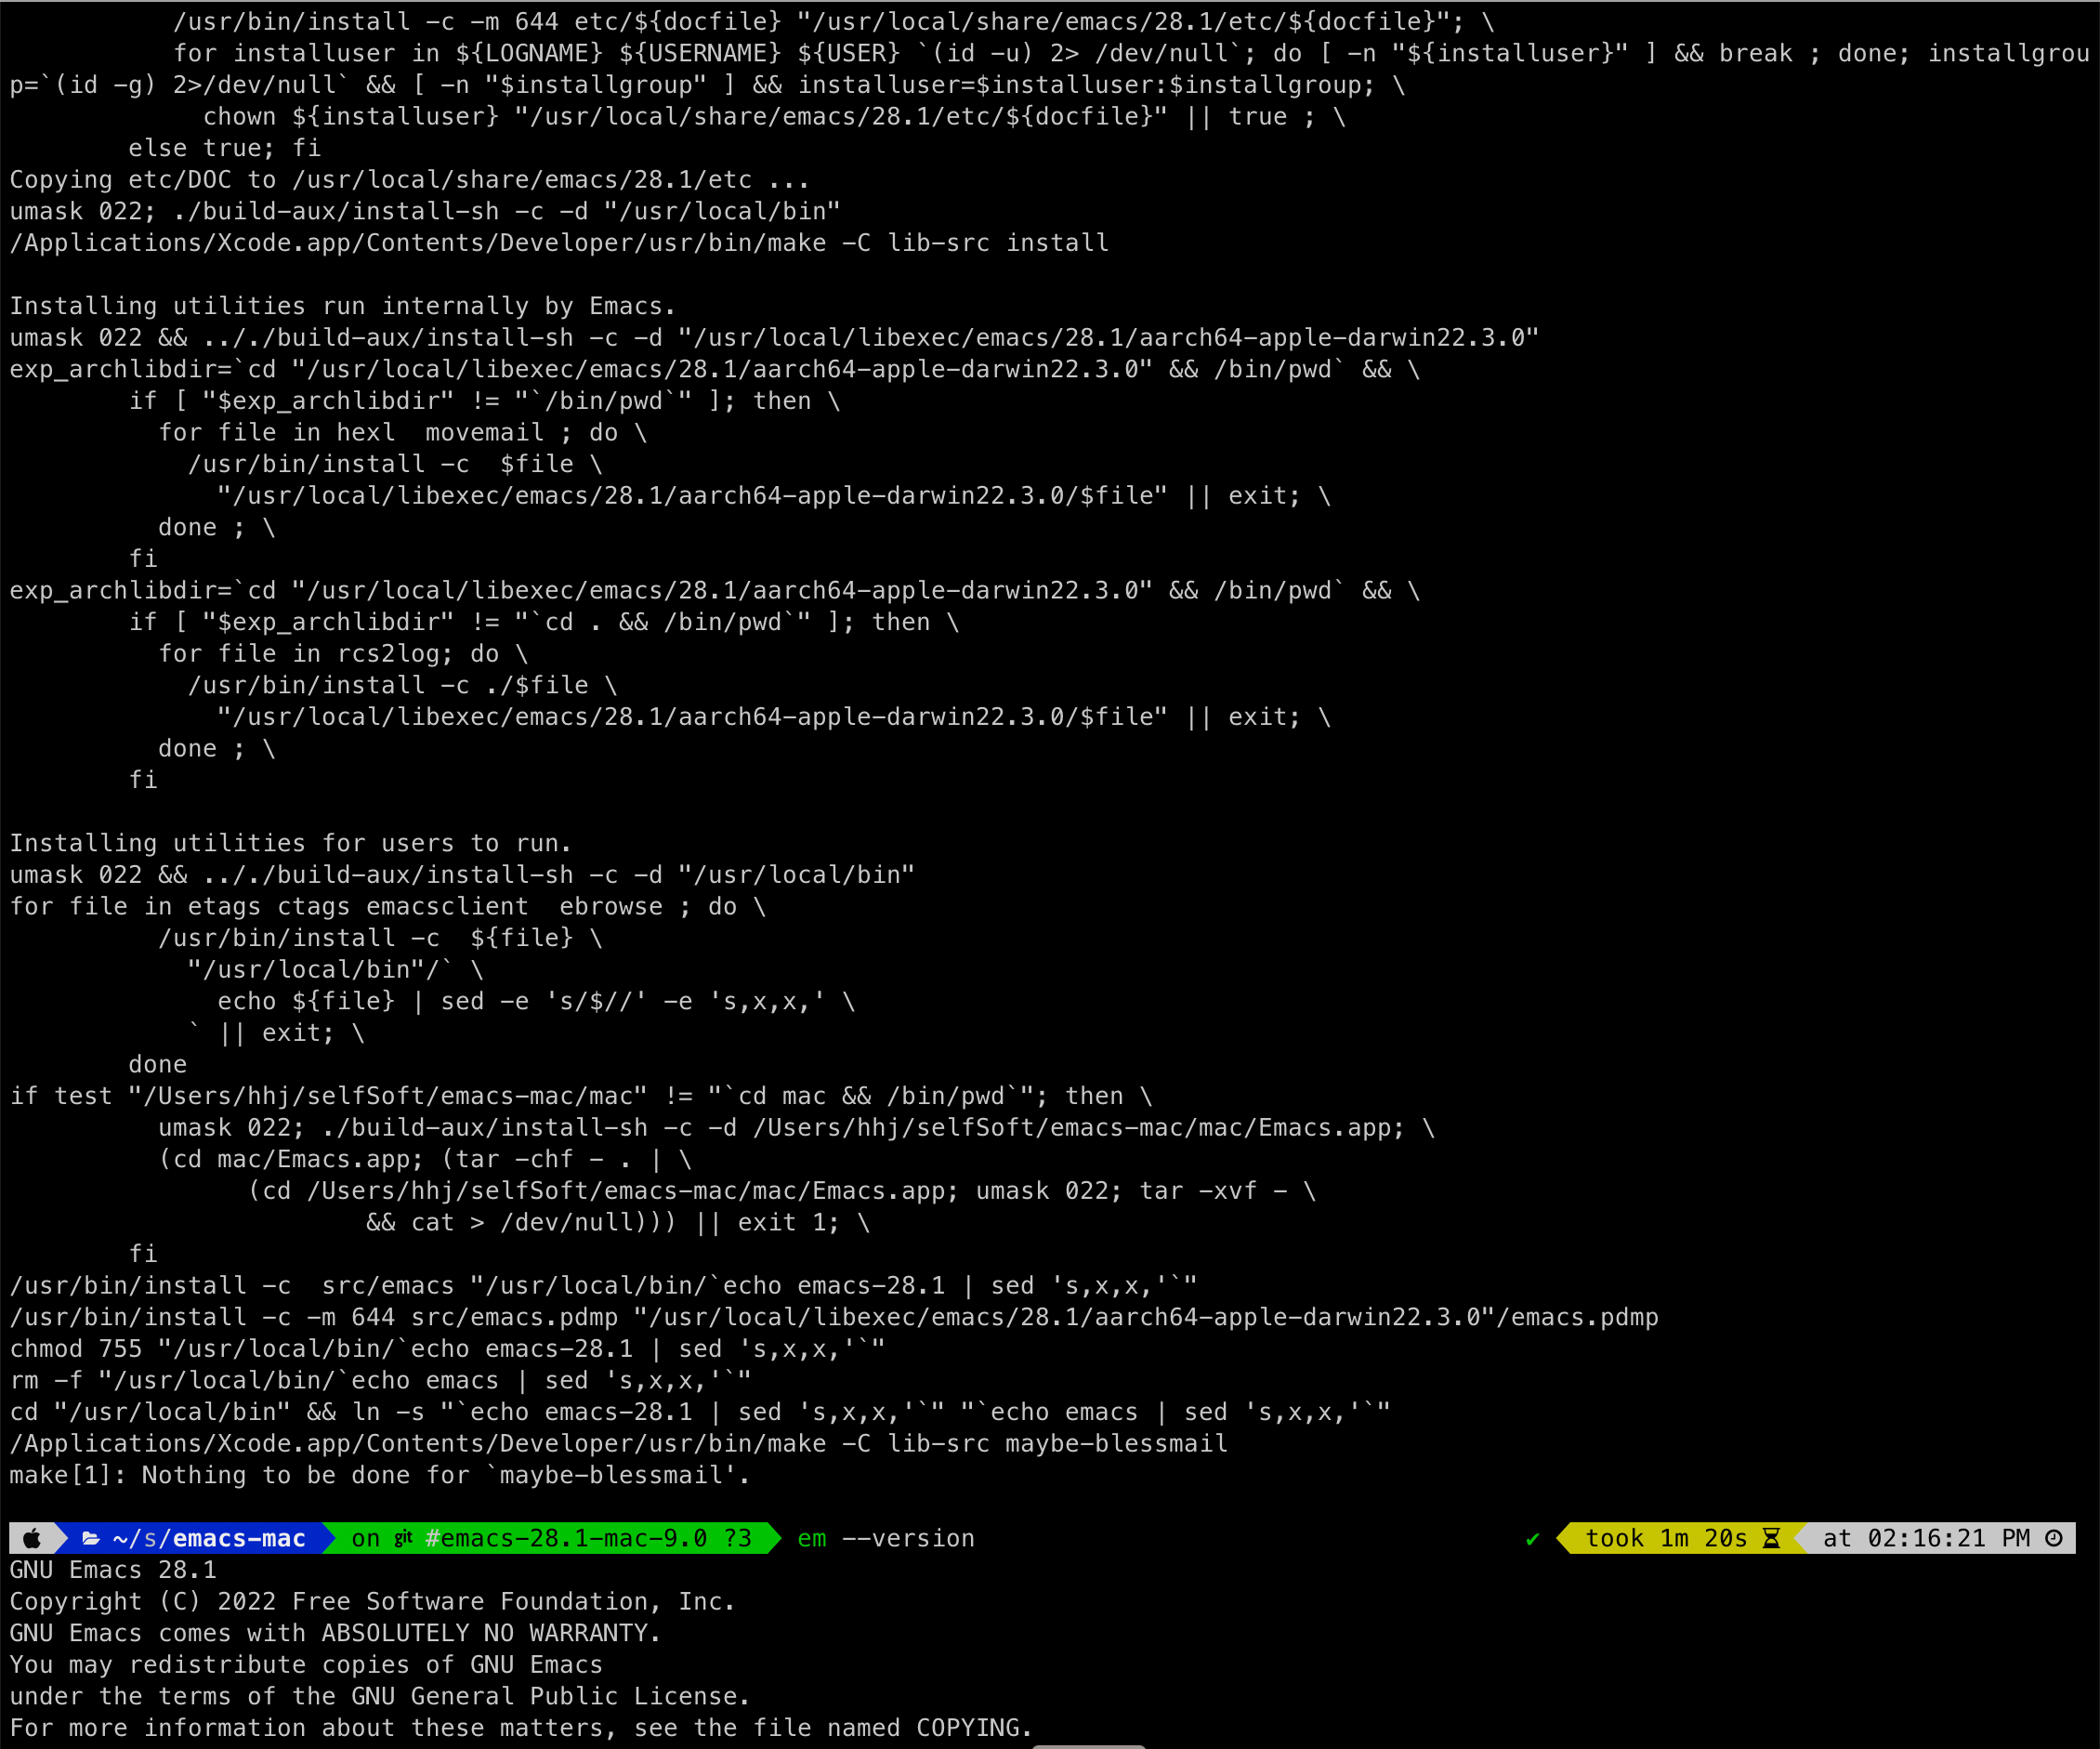
\includegraphics[width=.9\linewidth]{./pic/readme_20230208_142554.png}
\begin{itemize}
\item 今天又尝试安装Xcode之后再构建一遍,但是没有成功.可能本身参考有些年代,另外自己还完全不通这个部分,所以暂时放一放.改天有机会可以再回来研究一下,错在哪里,我如何才可能构建出自己的版本.
\end{itemize}

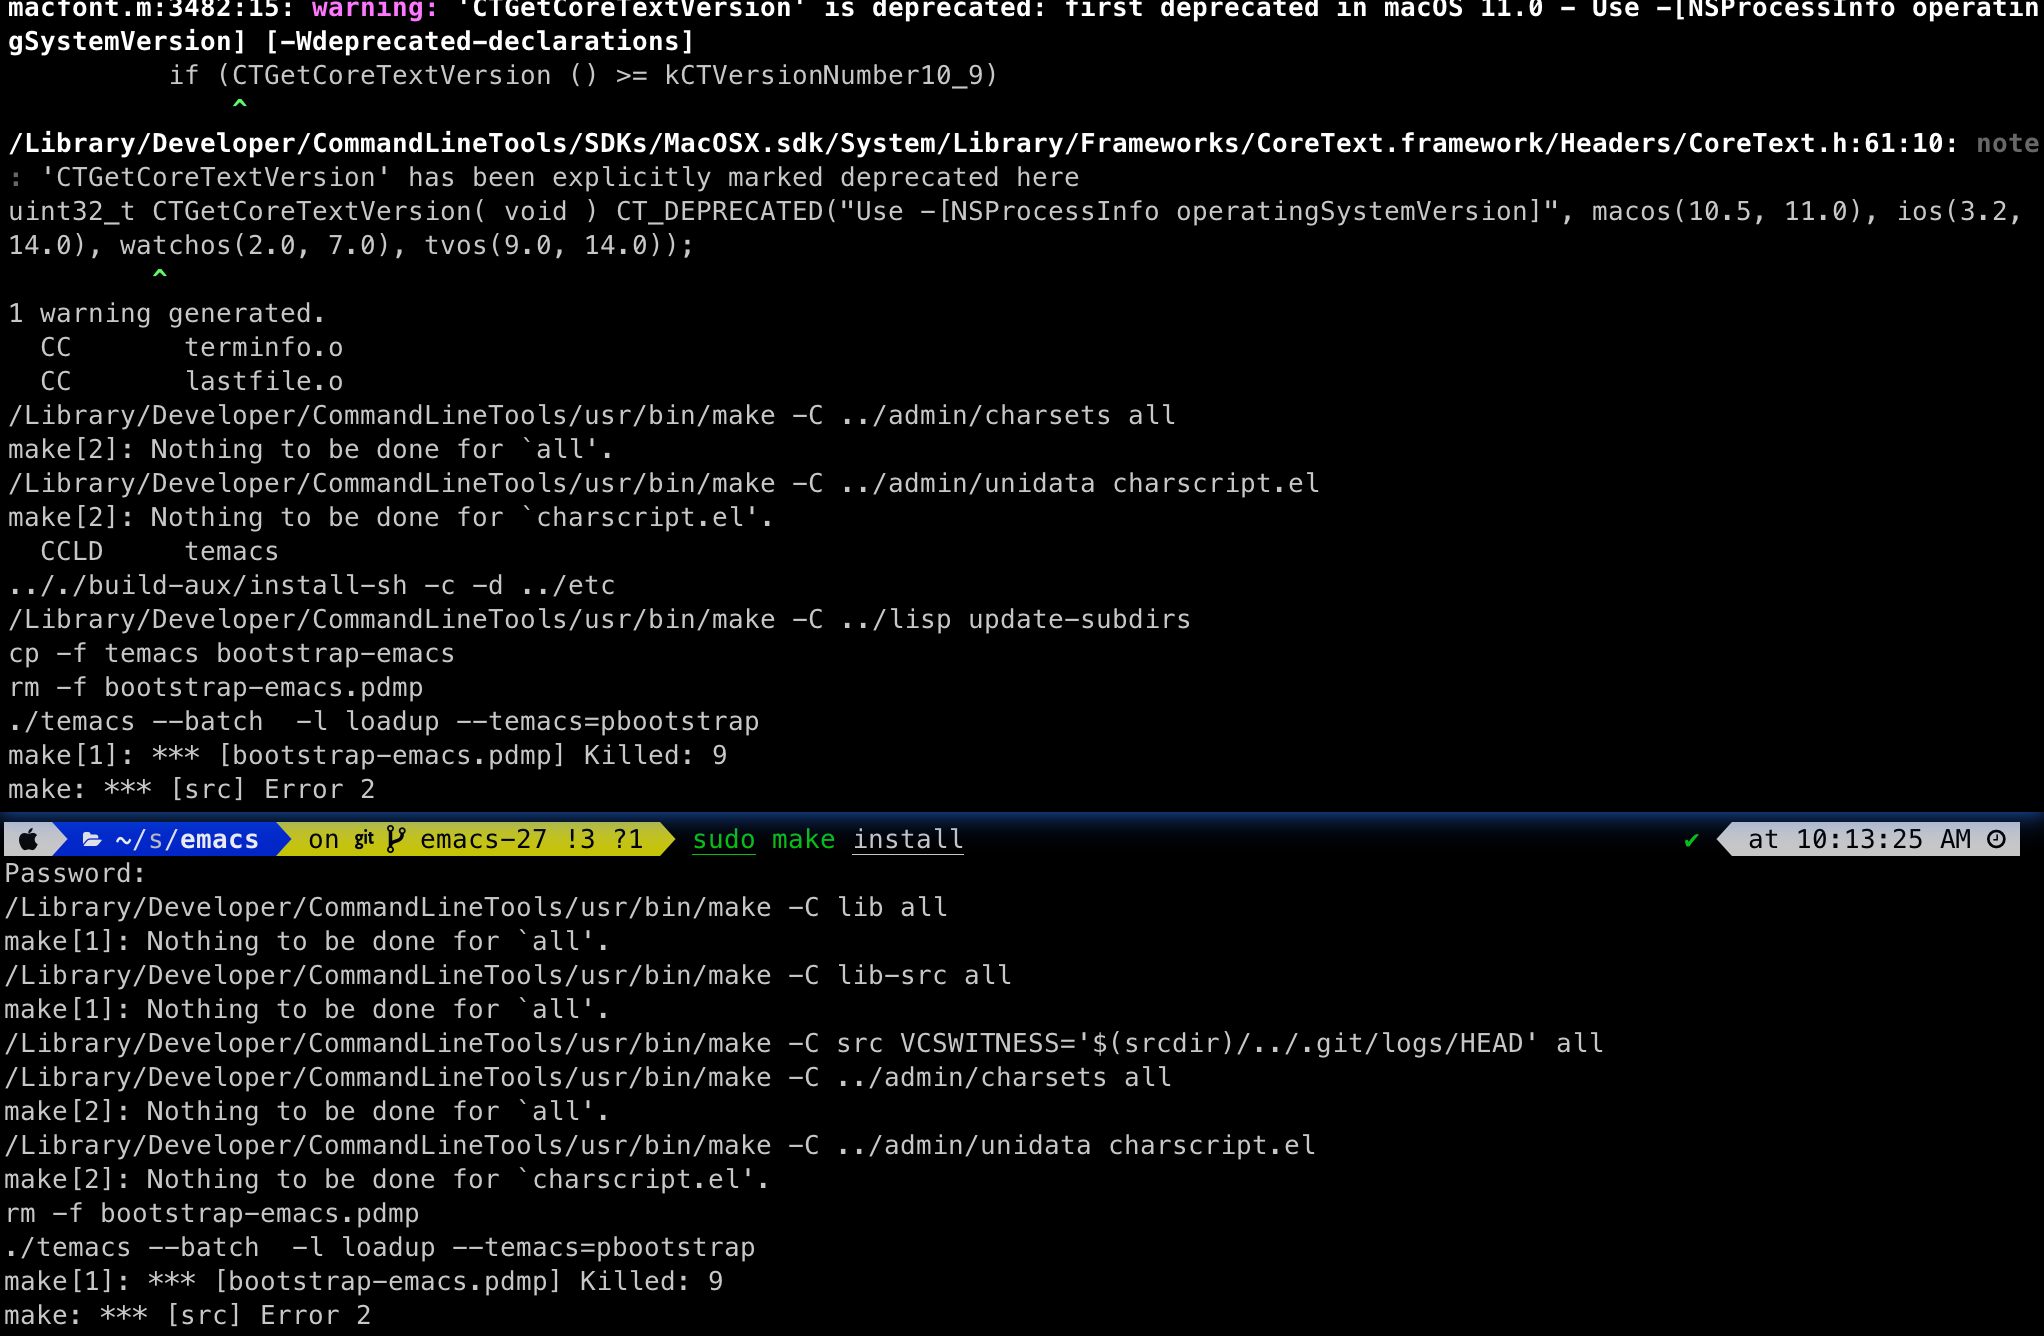
\includegraphics[width=.9\linewidth]{./pic/readme_20230208_102317.png}
\begin{itemize}
\item 上面又成为一个需要改的东西: 就是系统下如何从剪贴板自动生成写入文件 org-mode M-s
\item 然后看见这里说可以自己构建一个,连Xcode也没有安装,就跑去构建了,当然不成功。这段时间太忙,XCode要的空间太大了,暂时还不想。等改天有机会的时候倒是可以一试的
\begin{itemize}
\item \url{https://stuff-things.net/2020/12/28/building-emacs-27-dot-1-on-macos-big-sur/}
\end{itemize}
\item added key-bindings for opening from VSCode/Android Studio of current emacs buffer. 
\begin{itemize}
\item VSC Emacs can locate to each othr to correct row and col.
\item Android Studio could open current emacs buffer. but not to the row nor col.
\end{itemize}
\item I liked recently configued Visual studio 2019 one-dark-pro theme, want to configue it for emacs, but ended up with any permission denied, renaming emacs initiating bug. reverted back for daily use, and may look into that bug for later reference.
\item will reconfigure one-dark-pro theme later.
\item fixed legency java-mode highlighing issue which I did not fix for years. Has been able to treat java-mode as java-mode Instead of using it as csharp-mode. Can not separate java-mode snippets from csharp-mode's.
\end{itemize}
\subsection{BUG statement and partial fix}
\label{sec-2-3}
\begin{itemize}
\item in java-mode, the code style I expected is as followed:
\end{itemize}
\begin{minted}[fontsize=\scriptsize,linenos=false]{java}
class node {
    int v ;
    public node() {
        if (a > 0) // I don't want { } blocks when I have only one line statement inside blocks
     // a = 17;    // before fix:
            a = 17;   // now it can auto-indent
        b = 20;
        while (true)  // same auto indents here
            j++;
    }
}
class dklfjdj {|} // <<==== current un-auto-expanded version, bug right now for java-mode
class dklfjdj { 
    | // <<==== expected feature: once I typed '{', '}' will be autopaired(it does), but also auto-expand and cursor moves and indents directly to where I expect
}
\end{minted}
\begin{itemize}
\item if while if while one line statement autoindent without \{\} fixed today for java-mode, but for kotlin-mode, this bug consists, make coders/programmers nuts.
\end{itemize}
\begin{minted}[fontsize=\scriptsize,linenos=false]{java}
fun getStringLength(obj: Any): Int? {
    if (obj is String)
    return obj.length  // <<<<===== BUG: need to fix auto-indent here for if else while etc without {} 

    if (obj is String) {
        return obj.length
    }
    // 在离开类型检测分支后,`obj` 仍然是 `Any` 类型
    return null
}
fun dslfkj { // kotlin-mode, unlike java-mode, this feature works charming
    val a = 1720 
}
\end{minted}
\begin{itemize}
\item The \{|\} can NOT auto-expand still bugs me a lot, I don't want to switch back to java-mode yet unless bug fixed and it auto-pands.
\item java minor bug: Debugger entered--Lisp error: (void-function company-clear-completion-rules): this bug I will look into it recently, and expect it to be fixed so I could switch java-mode from csharp-mode as soon as possible.
\item \textbf{csharp-mode} has been the one that works perfectly for these two features, \{\} auto expand, also if while one line statement autoindent without \{\}, so I used csharp-mode as java mode.
\end{itemize}
\section{References}
\label{sec-3}
\begin{itemize}
\item \url{https://github.com/redguardtoo/emacs.d}
\end{itemize}

\section{windows 10 下面的 toggle-input-method 不 work: 想要绑定到一个方便使用的銉上面,另外 posframe (+ point 1)只想加上下,不想加左右。}
\label{sec-4}
\begin{itemize}
\item 有个想要打开文件时,不能C-a 到根目录的 bug:
\item 激活中文必须 M-x:pyim-activate; 切换成英文可以 either M-x:pyim-deactivate 或者是 C-\\
\item 再激活中文又必须是 M-x:pyim-activate
\item 需要一个简单的键绑定,帮助自己方便地切换到中文:而不是每次都得M-x:pyim-activate 太麻烦,易输入错误
\end{itemize}

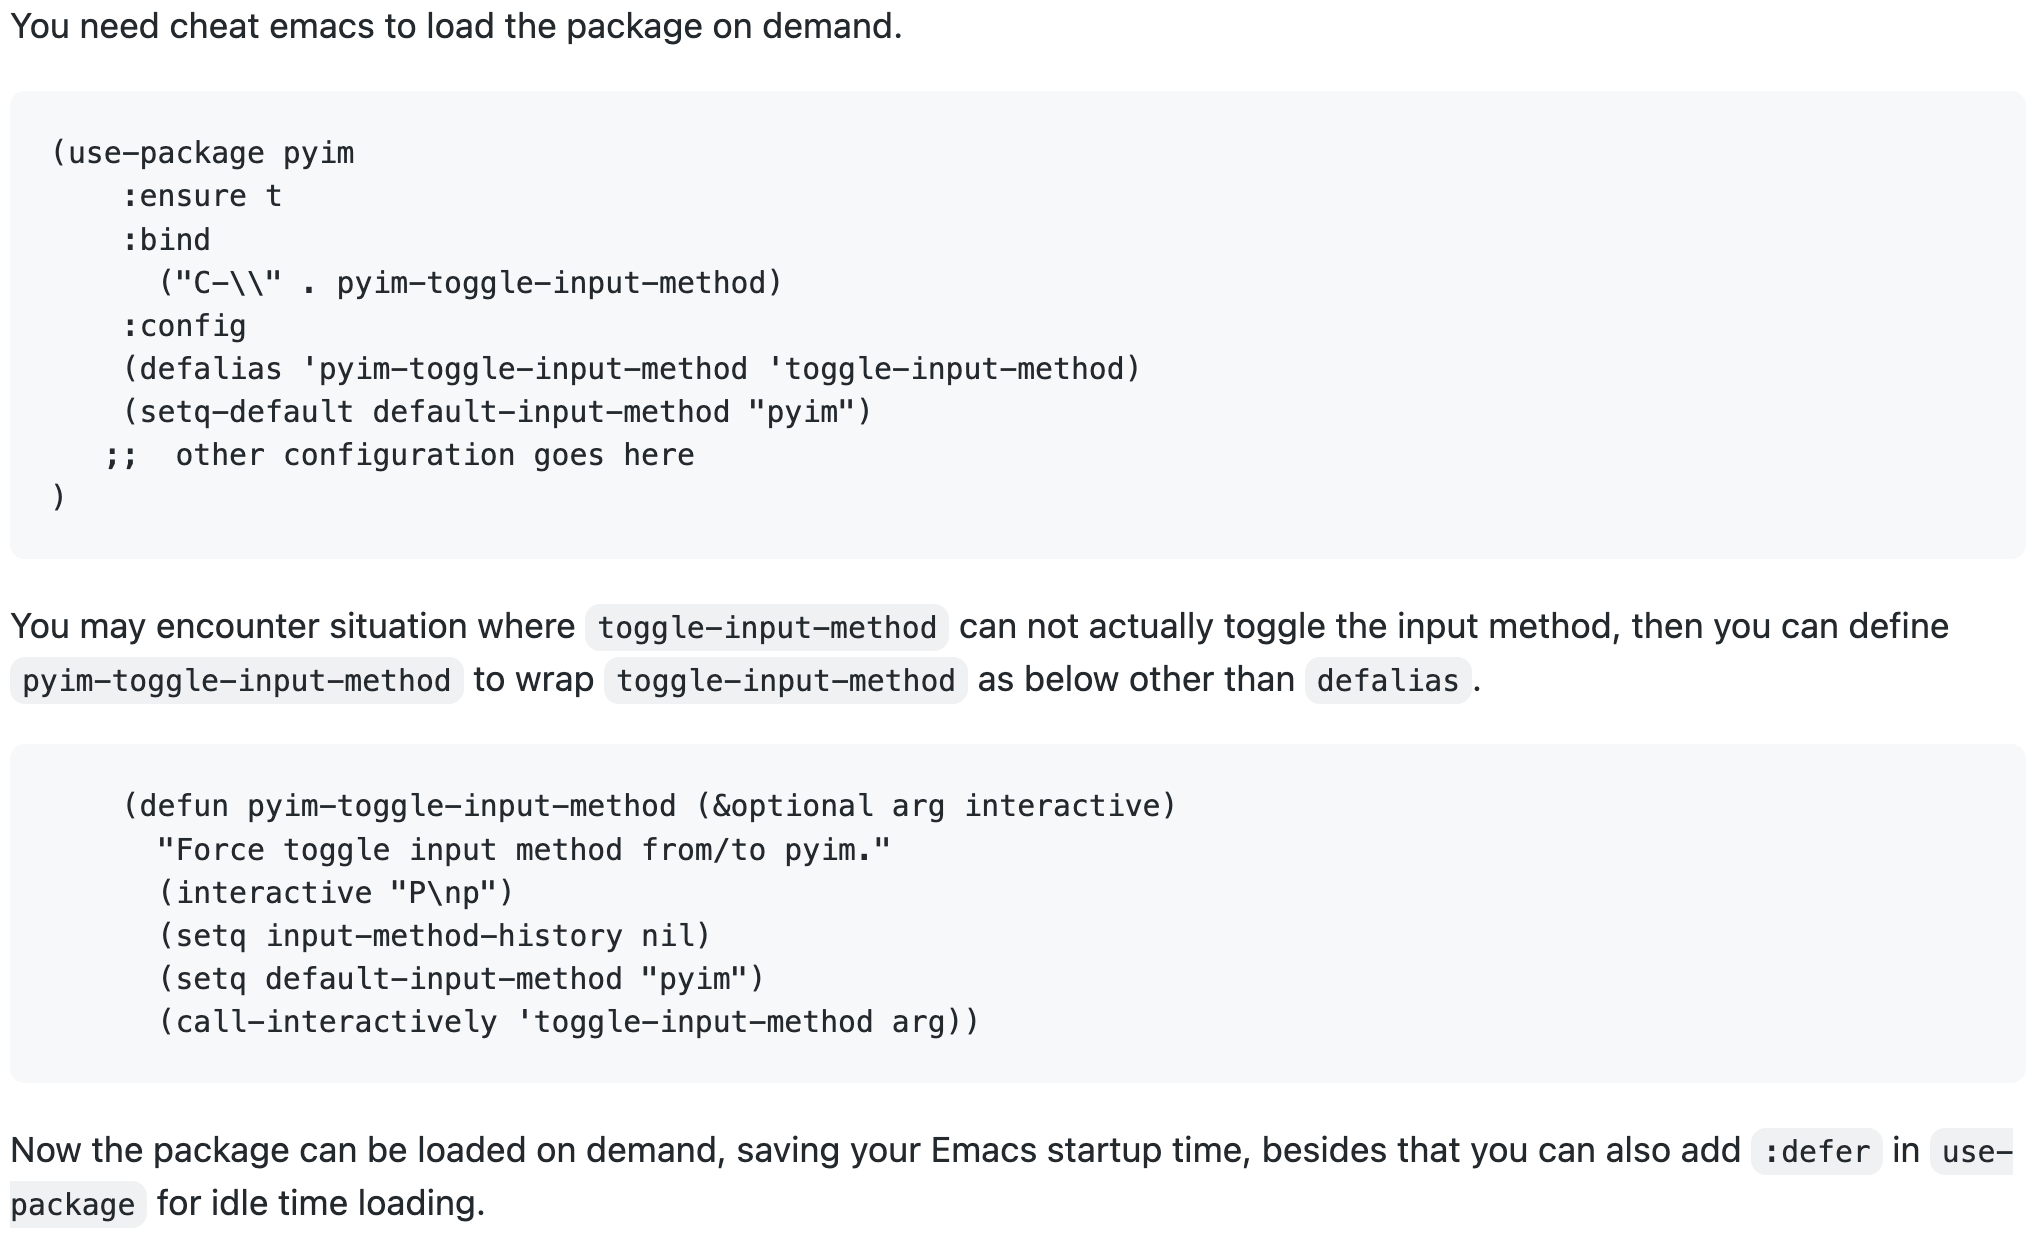
\includegraphics[width=.9\linewidth]{./pic/readme_20230226_130117.png}
% Emacs 28.2 (Org mode 8.2.7c)
\end{document}